

\tikzset{every picture/.style={line width=0.75pt}} %set default line width to 0.75pt        

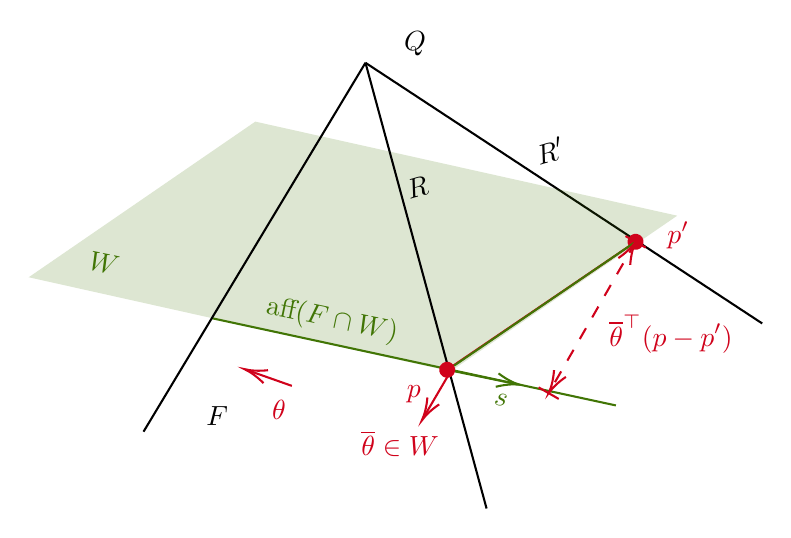
\begin{tikzpicture}[x=0.75pt,y=0.75pt,yscale=-1,xscale=1]
%uncomment if require: \path (0,300); %set diagram left start at 0, and has height of 300

%Straight Lines [id:da601159494474153] 
\draw [color={rgb, 255:red, 65; green, 117; blue, 5 }  ,draw opacity=1 ]   (329.04,218.1) -- (296.21,211.32) ;
\draw [shift={(331,218.5)}, rotate = 191.67] [color={rgb, 255:red, 65; green, 117; blue, 5 }  ,draw opacity=1 ][line width=0.75]    (10.93,-3.29) .. controls (6.95,-1.4) and (3.31,-0.3) .. (0,0) .. controls (3.31,0.3) and (6.95,1.4) .. (10.93,3.29)   ;
%Straight Lines [id:da16736332779785668] 
\draw    (256.86,63.41) -- (448,189) ;
%Shape: Parallelogram [id:dp029836882863379488] 
% [color={rgb, 255:red, 65; green, 117; blue, 5 }
\draw  [draw opacity=0][fill={rgb, 255:red, 65; green, 117; blue, 5 }  ,fill opacity=0.18 ] (203.78,91.76) -- (407.06,137.08) -- (297.88,212.07) -- (94.61,166.75) -- cycle ;
%Straight Lines [id:da1500138763319412] 
\draw    (256.86,63.41) -- (315.2,278.15) ;
%Straight Lines [id:da601483538224197] 
\draw [color={rgb, 255:red, 65; green, 117; blue, 5 }  ,draw opacity=1 ]   (377.5,228.5) -- (183,186.5) ;
%Straight Lines [id:da6958390303159552] 
\draw [color={rgb, 255:red, 208; green, 2; blue, 27 }  ,draw opacity=1 ]   (296.21,211.32) -- (387,149.67) ;
\draw [shift={(387,149.67)}, rotate = 325.82] [color={rgb, 255:red, 208; green, 2; blue, 27 }  ,draw opacity=1 ][fill={rgb, 255:red, 208; green, 2; blue, 27 }  ,fill opacity=1 ][line width=0.75]      (0, 0) circle [x radius= 3.35, y radius= 3.35]   ;
\draw [shift={(296.21,211.32)}, rotate = 325.82] [color={rgb, 255:red, 208; green, 2; blue, 27 }  ,draw opacity=1 ][fill={rgb, 255:red, 208; green, 2; blue, 27 }  ,fill opacity=1 ][line width=0.75]      (0, 0) circle [x radius= 3.35, y radius= 3.35]   ;
%Straight Lines [id:da2936586396129306] 
\draw    (256.86,63.41) -- (149.93,241.15) ;
%Straight Lines [id:da3259773897357544] 
\draw [color={rgb, 255:red, 65; green, 117; blue, 5 }  ,draw opacity=1 ]   (299.55,209.32) -- (387,149.67) ;
%Straight Lines [id:da3403685536850527] 
\draw [color={rgb, 255:red, 208; green, 2; blue, 27 }  ,draw opacity=1 ]   (297.88,212.07) -- (285.01,234.03) ;
\draw [shift={(284,235.76)}, rotate = 300.37] [color={rgb, 255:red, 208; green, 2; blue, 27 }  ,draw opacity=1 ][line width=0.75]    (10.93,-3.29) .. controls (6.95,-1.4) and (3.31,-0.3) .. (0,0) .. controls (3.31,0.3) and (6.95,1.4) .. (10.93,3.29)   ;
%Straight Lines [id:da34888955494418983] 
\draw [color={rgb, 255:red, 208; green, 2; blue, 27 }  ,draw opacity=1 ] [dash pattern={on 4.5pt off 4.5pt}]  (387,149.67) -- (345.12,222.59) ;
\draw [shift={(345.12,222.59)}, rotate = 299.87] [color={rgb, 255:red, 208; green, 2; blue, 27 }  ,draw opacity=1 ][line width=0.75]    (0,5.59) -- (0,-5.59)(10.93,-3.29) .. controls (6.95,-1.4) and (3.31,-0.3) .. (0,0) .. controls (3.31,0.3) and (6.95,1.4) .. (10.93,3.29)   ;
\draw [shift={(387,149.67)}, rotate = 119.87] [color={rgb, 255:red, 208; green, 2; blue, 27 }  ,draw opacity=1 ][line width=0.75]    (0,5.59) -- (0,-5.59)(10.93,-3.29) .. controls (6.95,-1.4) and (3.31,-0.3) .. (0,0) .. controls (3.31,0.3) and (6.95,1.4) .. (10.93,3.29)   ;
\draw [color={rgb, 255:red, 208; green, 2; blue, 27 }  ,draw opacity=1 ]   (221.38,219.07) -- (200.39,211.67) ;
\draw [shift={(198.5,211)}, rotate = 19.44] [color={rgb, 255:red, 208; green, 2; blue, 27 }  ,draw opacity=1 ][line width=0.75]    (10.93,-3.29) .. controls (6.95,-1.4) and (3.31,-0.3) .. (0,0) .. controls (3.31,0.3) and (6.95,1.4) .. (10.93,3.29)   ;

% Text Node
\draw (209.34,172.66) node [anchor=north west][inner sep=0.75pt]  [color={rgb, 255:red, 65; green, 117; blue, 5 }  ,opacity=1 ,rotate=-11.74] [align=left] {aff$\displaystyle ( F\cap W)$};
% Text Node
\draw (274,47) node [anchor=north west][inner sep=0.75pt]   [align=left] {$\displaystyle Q$};
% Text Node
\draw (123.7,152.12) node [anchor=north west][inner sep=0.75pt]  [color={rgb, 255:red, 65; green, 117; blue, 5 }  ,opacity=1 ,rotate=-11.74] [align=left] {$\displaystyle W$};
% Text Node
\draw (178.67,227.33) node [anchor=north west][inner sep=0.75pt]   [align=left] {$\displaystyle F$};
% Text Node
\draw (273.73,119.53) node [anchor=north west][inner sep=0.75pt]  [rotate=-343.64] [align=left] {$\displaystyle R$};
% Text Node
\draw (275.33,217.33) node [anchor=north west][inner sep=0.75pt]  [color={rgb, 255:red, 208; green, 2; blue, 27 }  ,opacity=1 ] [align=left] {$\displaystyle p$};
% Text Node
\draw (400.83,138.33) node [anchor=north west][inner sep=0.75pt]  [color={rgb, 255:red, 208; green, 2; blue, 27 }  ,opacity=1 ] [align=left] {$\displaystyle p'$};
% Text Node
\draw (335.73,101.53) node [anchor=north west][inner sep=0.75pt]  [rotate=-343.64] [align=left] {$\displaystyle R'$};
% Text Node
\draw (318.51,220.49) node [anchor=north west][inner sep=0.75pt]  [color={rgb, 255:red, 65; green, 117; blue, 5 }  ,opacity=1 ,rotate=-11.74] [align=left] {$\displaystyle s$$ $};
% Text Node
\draw (253.39,239.44) node [anchor=north west][inner sep=0.75pt]  [color={rgb, 255:red, 208; green, 2; blue, 27 }  ,opacity=1 ,rotate=0] [align=left] {$\displaystyle \overline{\theta } \in W$$ $};
% Text Node
\draw (372.85,183.32) node [anchor=north west][inner sep=0.75pt]  [color={rgb, 255:red, 208; green, 2; blue, 27 }  ,opacity=1 ,rotate=-0] [align=left] {$\displaystyle \overline{\theta }^{\top }( p-p')$$ $};
% Text Node
\draw (210.39,224.44) node [anchor=north west][inner sep=0.75pt]  [color={rgb, 255:red, 208; green, 2; blue, 27 }  ,opacity=1 ,rotate=0] [align=left] {$\displaystyle \theta $$ $};

\end{tikzpicture}